\documentclass[11pt,a4paper]{extarticle}
\usepackage[utf8]{inputenc}
\usepackage[T1]{fontenc}
\usepackage[hidelinks]{hyperref} 
\usepackage[russian,english]{babel}
\usepackage{amsthm}
\usepackage{listings}
\usepackage{amsmath}
\usepackage{amsfonts}
\usepackage{amssymb}
\usepackage{xcolor,colortbl}
\usepackage{graphicx}
\usepackage{subcaption}
\usepackage{fullpage}
\usepackage[nottoc,numbib]{tocbibind}

\definecolor{Gray}{gray}{0.95}
\definecolor{Red}{rgb}{0.80,0.5,0.5}
\definecolor{Green}{rgb}{0.6,0.8,0.6}

\newenvironment{compactlist}{
\begin{list}{{$\bullet$}}{
\setlength\partopsep{0pt}
\setlength\parskip{0pt}
\setlength\parsep{0pt}
\setlength\topsep{0pt}
\setlength\itemsep{0pt}
}}{
\end{list}
}


\begin{document}
\selectlanguage{russian}
\begin{titlepage}
	\begin{centering}
		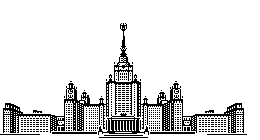
\includegraphics{img/msu}\\
		\large{
			\textbf{Московский государственный университет имени М.В. Ломоносова}\\
			Факультет вычислительной математики и кибернетики\\
			Кафедра интеллектуальных информационных технологий\\[4cm]
		}
		\Large{
			Гончаренко Дмитрий Александрович\\[0.9cm]
		}
		\Large{
			\textbf{Алгоритм изменения времени суток на изображении}\\
			% \textbf{Research of Changing The Time of Day on Images}\\
		}
		\rule[0.3cm]{14cm}{0.02cm}\\[1cm]
		\large{
			ВЫПУСКНАЯ КВАЛИФИКАЦИОННАЯ РАБОТА\\[4cm]
		}
	\end{centering}
	\begin{flushright}
		\large{
			\textbf{Научный руководитель:}\\ К.С. Зипа\\
		}
	\end{flushright}
	\begin{center}
		\vfill
		\large{
			Москва, 2019
		}
	\end{center}
\end{titlepage}

\begin{abstract}
	Алгоритм изменения времени суток на изображении относится к классу задач машинного обучения по переносу
	изображений\footnote{\textbf{Перенос изображений} (англ. \textbf{image translation}, или \textbf{image transfering}) -- подвид технологии переноса обучения, позволяющий сохранять и объединять локальные признаки изображений}.
	Данная сфера значительное продвинулась благодаря современным вычислительным возможностям, в частности переносе обучения на графические процессоры, GPU.
	За последние несколько лет появилось немало исследовательских работ на тему переноса изображений, стилей и колоризации.
	В данной работе рассматриваются современные подходы к переносу изображений на примере изменения времени суток на изображении.
	Проводится описание нейросетевых моделей и сравнительный анализ серии экспериментов обучения.
\end{abstract}

\selectlanguage{english}
\begin{abstract}
	The algorithm of changing the time of the day on images is a subclass of Machine Learning problems of image translation.
	This area has advanced significantly due to the modern computing capabilities, in particular the training transfer on GPUs.
	Over the past few years, many research papers have appeared on the subject of images translation, styles transfering and coloring.
	This research reveals modern approaches of image translation on the example of changing the time of day on the image.
	A description of the neural network models and a comparative quality analysis of a series of training experiments are carried out.
\end{abstract}

\selectlanguage{russian}

\newpage
\tableofcontents
\newpage

\section{Введение}
	\textbf{Перенос изображений} -- 
\section{Постановка задачи}

\section{Обзор существующих решений}

\section{Исследование и построение решения задачи}

\section{Описание практической части}

\section{Заключение}

\section{Список цитируемой литературы}

\section{Предметная область}

\begin{thebibliography}{00}

	\bibitem{tag}
	\textbf{Author}.
	\emph{Article Name}.
	Sony Computer Entertainment, Santa Monica, USA,
	Date, 2004.


\end{thebibliography}

\end{document}